\section{Evaluation}

We ran our tests on the QEMU \cite{qemu} hypervisor on top of Linux 4.11.8,
with hardware virtualization enabled (using KVM.) In the benchmarks described
below, all virtual machines were launched with two processors, and a varying
amount of RAM. Since MLCache's main goal is to make smarter cache eviction
decisions, most of our interest lies in benchmarks where the size of the page
cache can potentially outgrow the amount of memory available in the system.

We developed two different benchmarks to test MLCache:

\begin{itemize}
  \item \textbf{\texttt{cscope}.} This benchmark consists of running \texttt{make cscope}
    inside the Linux kernel source tree. \texttt{cscope} is a source code indexing
    tool which allows developers to quickly find C symbol definitions, function call
    sites, pattern matching, among others. The purpose of this benchmark is to evaluate
    how well MLCache performs in a workload that is primarily sequential (scanning of
    source files.)
  \item \textbf{\texttt{pgbench}.} This benchmark consists of running the \texttt{pgbench}
    utility on a database that is a lot larger than available memory. \texttt{pgbench} is a bechmarking
    tool for the PostgreSQL database. It is able to perform a variety of tests, some of
    which based on the TPC-B database benchmark \cite{tpcb}.  The goal of this test is to
    understand how MLCache can potentially help a common scenario in commercial applications
    (a dedicated database server.)
\end{itemize}

\label{fig:cscope}
\begin{figure}[h]
	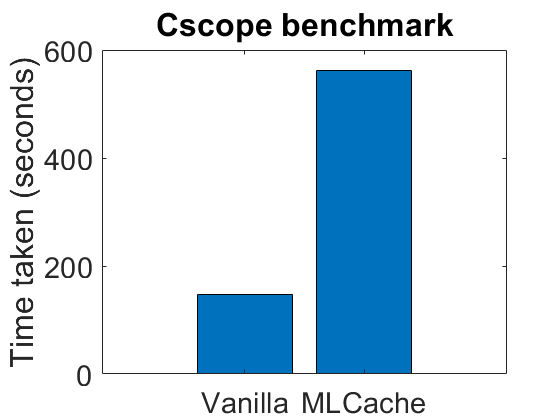
\includegraphics[scale=0.4]{img/cscope_results_bigger.png}
	\caption{Cscope benchmark results for the unmodified Linux kernel versus our MLCache prototype, ran on a VM with 256MB of RAM.}
\end{figure}

The results from the \textbf{cscope} benchmark give us some sense of the
overhead caused by our implementation, as the current Linux implementation does
not benefit very much from caching for this benchmark. We can see that the time
taken was about 3x larger on MLCache. This is not surprising, as we have to update
each page's scores in the cache on every reference, as well as doing a linear
scan over Linux's linked list on eviction. Additionally, Linux is already very optimized
for the linear scan scenario, reading blocks ahead of time when a page is requested.
Thus, MLCache only adds overhead for score maintenance in this case and performance
is greatly affected.

\label{fig:pg}


\begin{figure}[h]
	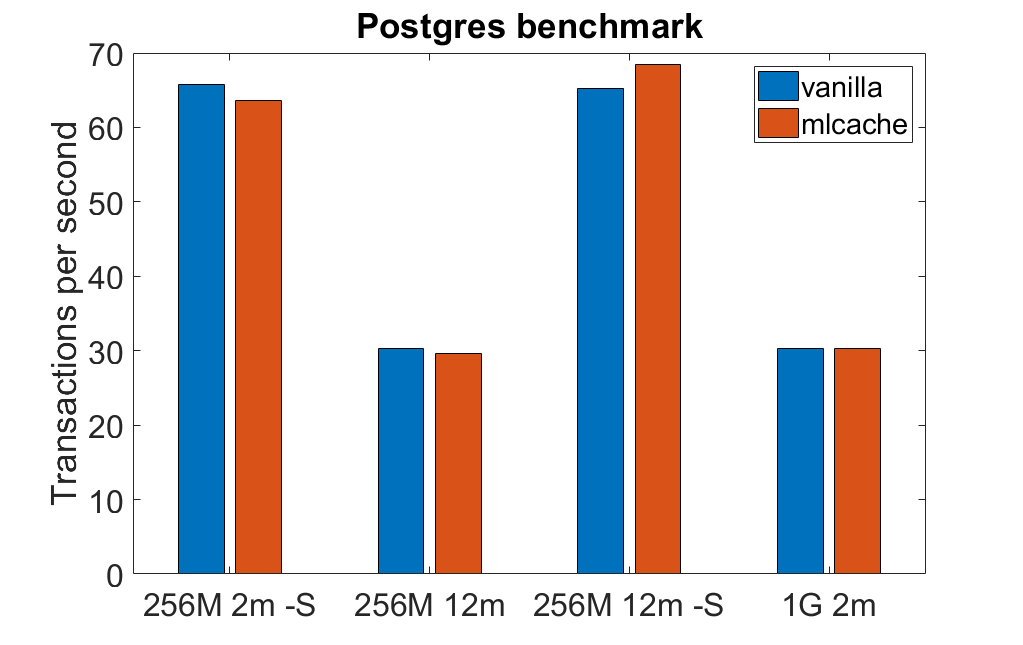
\includegraphics[scale=0.3]{img/postgres_results_bigger.png}
	\caption{Postgres benchmark results for the unmodified Linux kernel versus our MLCache prototype, with different RAM sizes. The -S command means just reads, no writes.}
\end{figure}

Our results from the \textbf{pgbench} benchmark show us that even with the extra
machinery we have built on top of Linux, we achieve similar performance,
especially as memory decreases and on longer runs. This is probably due to the
current implementation having to develop new scores from scratch on every run,
and so reaching accurate scores takes some time. After 12 minutes, however, our
design starts to outperform Linux. This is relatively fast, since training
would ideally be done only once, and the rest is online learning. We should
note that our implementation takes advantage of smaller memory sizes due to the
increased amount of evictions done: without any evictions, our design is entirely
overhead.

As a small experiment, we also tested how our implementation fared when
evicting the lowest score (best) pages every time. For the \textbf{cscope} benchmark, it
took about 3 hours to complete. This gave us some reassurance that our algorithm,
although not ideal, is in the right direction compared to a completely naive
implementation.
